\documentclass[11pt,a4paper,oldfontcommands, oneside]{memoir}
\usepackage[utf8]{inputenc}
\usepackage[T1]{fontenc}
\usepackage{microtype}
%\usepackage{hyperref}%
\usepackage[dvips]{graphicx}
\usepackage{xcolor}
\usepackage{times}
\usepackage{algorithm}
\usepackage{algpseudocode}
\usepackage{amsmath}
\usepackage{MnSymbol}%
\usepackage{wasysym}%

\usepackage[
breaklinks=true,colorlinks=true,
%linkcolor=blue,urlcolor=blue,citecolor=blue,% PDF VIEW
linkcolor=black,urlcolor=black,citecolor=black,% PRINT
bookmarks=true,bookmarksopenlevel=2]{hyperref}

\usepackage{geometry}
% PDF VIEW
% \geometry{total={210mm,297mm},
% left=25mm,right=25mm,%
% bindingoffset=0mm, top=25mm,bottom=25mm}
% PRINT
\geometry{total={210mm,297mm},
left=20mm,right=20mm,
bindingoffset=10mm, top=25mm,bottom=25mm}

\OnehalfSpacing
%\linespread{1.3}

%%% CHAPTER'S STYLE
%\chapterstyle{bianchi}
%\chapterstyle{ger}
\chapterstyle{madsen}
%\chapterstyle{ell}
%%% STYLE OF SECTIONS, SUBSECTIONS, AND SUBSUBSECTIONS
\setsecheadstyle{\Large\bfseries\sffamily\raggedright}
\setsubsecheadstyle{\large\bfseries\sffamily\raggedright}
\setsubsubsecheadstyle{\bfseries\sffamily\raggedright}

\setlength{\oddsidemargin}{5mm}
\setlength{\evensidemargin}{5mm}
%%% STYLE OF PAGES NUMBERING
%\pagestyle{companion}\nouppercaseheads 
%\pagestyle{headings}
%\pagestyle{Ruled}
\pagestyle{plain}
\makepagestyle{plain}
\makeevenfoot{plain}{\thepage}{}{}
\makeoddfoot{plain}{}{}{\thepage}
\makeevenhead{plain}{}{}{}
\makeoddhead{plain}{}{}{}


\maxsecnumdepth{section} % chapters, sections, and subsections are numbered
\maxtocdepth{section} % chapters, sections, and subsections are in the Table of Contents


%%%---%%%---%%%---%%%---%%%---%%%---%%%---%%%---%%%---%%%---%%%---%%%---%%%

\begin{document}

%%%---%%%---%%%---%%%---%%%---%%%---%%%---%%%---%%%---%%%---%%%---%%%---%%%
%   TITLEPAGE
%
%   due to variety of titlepage schemes it is probably better to make titlepage manually
%
%%%---%%%---%%%---%%%---%%%---%%%---%%%---%%%---%%%---%%%---%%%---%%%---%%%
\thispagestyle{empty}

{%%%
\sffamily
\centering
\Large

~\vspace{\fill}

{\huge 
Hand Tracking with Microsoft Kinect v2 and Leap Motion\\
}
\vspace{1.5cm}
{\Large
Practical Course of Data Fusion}



\vspace{5cm}

{\large
Hendrik Bitzmann \\
Hanna Holderied \\
Christoph Rauterberg \\
Maximilian Weß
}


\vspace{\fill}
Jun. Prof. Marcus Baum\\
Institute for Applied Computer Sciences\\
University of G\"ottingen


September 2016

%%%
}%%%

\cleardoublepage
%%%---%%%---%%%---%%%---%%%---%%%---%%%---%%%---%%%---%%%---%%%---%%%---%%%
%%%---%%%---%%%---%%%---%%%---%%%---%%%---%%%---%%%---%%%---%%%---%%%---%%%

\tableofcontents*

%\clearpage

%%%---%%%---%%%---%%%---%%%---%%%---%%%---%%%---%%%---%%%---%%%---%%%---%%%
%%%---%%%---%%%---%%%---%%%---%%%---%%%---%%%---%%%---%%%---%%%---%%%---%%%

%Citation of Einstein paper~\cite{Einstein}.

\chapter{Introduction}
This project report is the result of the participation in the "Practical Course: Data Fusion" in the Summer Semester 2016.


The goal of this project was to construct a scene in a virtual reality in which a user is able to interact with an object using his or her hands and fingers. To achieve this goal we were given two kinds of sensors:
\begin{enumerate}
	\item A Microsoft Kinect v2\footnote{\url{https://developer.microsoft.com/de-de/windows/kinect/develop}} and
	\item A Leap Motion Sensor\footnote{\url{https://www.leapmotion.com/}}.
\end{enumerate}


The Microsoft Kinect v2 was released in 2014 and brings an infrared depth sensor, a RGB sensor and 3D motion tracking to the table. The last is especially important for this project. The Kinect can reach between 15 to 30 frames per second (fps).   \\
The Leap Motion sensor uses two monochromatic IR cameras and three infrared LEDs to observe a hemispherical area in front of the device and can reach up to 200fps.


In this report we will highlight our line of work to enable future research to be able to set up such an environment more quickly. 
Firstly, we will describe all steps that are necessary to achieve a working Kinect environment under Windows and Linux. We will then describe which algorithmic approaches we inferred and in the end chose to achieve the desired goals of this project. We will conclude by discussing our first approach for combining the sensor readings from the Kinect and the Leap Motion Sensor.


%Leap raus -> discussion/conclusion?
%The second device we tried to use is a Leap Motion, also with a build-in infrared camera. This is a small object you place in front of your keyboard and via tracking your hand gestures it allows you to control your PC, or like in our case a coffee machine.
%Unfortunately we did not have enough time to implement the usage of the Leap Motion completely, but we will share our few experiences anyway.
%We tried to use the Leap to increase the accuracy of the tracked motions.\\
%
%
%In the end we want to find out whether it is possible to use and fuse techniques like this to create a similar user experience with virtual reality compared to real world interactions. This could e.g. be used to evaluate the usability of several products.\\


\chapter{Methods}

\section{Setup}

\subsection{Configuration of the Kinect v2}
Firstly we have to emphasize that the Kinect sensors (Kinect v1 and Kinect v2) are provided by the Microsoft Cooperation and are therefore for development under the operating system Windows, nowdays preferrably Windows 10. All current solutions for Linux are community based.


There are solutions such as \emph{libfreenect}\footnote{\url{https://github.com/OpenKinect/libfreenect2}} which provide drivers for Linux - however, we could only achieve a working version of this with Ubuntu and not Arch Linux. To establish a working version of \emph{libfreenect} with the according Python-wrapper \emph{python-freenect2}\footnote{\url{https://github.com/OpenKinect/libfreenect/tree/master/wrappers/python}} took quite an amount of work - we would therefore discourage anyone from using the Linux drivers if time is dire.


Furthermore it is important to mention that you need to have an USB 3.0 port if you want to use the Kinect v2, otherwise it will not work. In addition you need moderate computation power. It turned out that a notebook with just HD4000 graphics is not suitable.


The first step for using the Kinect v2 under Windows is downloading the  official \emph{Kinect 2.0 Software Development Kit} from Microsoft for Windows\footnote{\url{https://www.microsoft.com/en-us/download/details.aspx?id=44561}}. The SDK includes many useful tools and examples. Next step should be starting the Kinect Configuration Verifier from the SDK browser, which will check the system requirements. Every check besides for the USB controller should be successful. In our experience, a warning for the USB port did not turn out to be a problem.\\

\subsection{Set up a working development environment}
We choose a running start by following the tutorial from [???] . This gave us a working development environment consisting of Unity3D, Visual Studio 2015 and the Kinect SDK, already with a working "Hello World" example.\\
Unity3d is a game development engine. It is a good choice for our application, because of ease which simple tasks can be executed. The import of assets into the project can be achieved via drag and drop and also linking scripts for event handling and update mechanisms to this assets is handled via drag and drop. The editing of scripts/code can be done in Visual Studio 2015, which is the state-of-the-art Windows IDE. We imported the source code into Unity3D and Visual Studio 2015, as a programming language we have chosen C\# - simply for convinience.


\subsection{Moving objects in a Virtual Reality}
First of all, we needed models for a Unity3D-scene. Patrick Harms provided us with a working \emph{Blender}-Model\footnote{Blender is the free and open source 3D creation suite.} of a coffe machine, written by one of his students.
\\
To first understand the combination between our C\# -Scripts and the Unity-Scene, we started out with simple spheres in a 3D-system. Those objects can be created very simple in Unity. Furthermore we found \emph{Blender}-model that represented Hands in a 3D-space\footnote{\url{https://clara.io/view/3e6923db-407c-4e0c-a253-2f564dfcd152}}. \\
After integrating these models in a Unity-Scene we were able to compute events: \\
We used a haptical feedback to emulate the proximity of the hands to the spheres created in the beginning. Whenever the hands were moving closer towards the sphere, the sphere itself would change its color - depending on the \emph{eucledian distance} to the \emph{mesh grid} of the hands. In the Unity-Scene, the 3D-Model of two hands consists of a mesh grid of coordinates for each hand, which represent the shape of the hands, and textures that is rendered over these mesh grids. 


To compute the proximity between a sphere and the hands, we could therefore simply compute the euclidian distance between the coordinates of the mesh grid and the coordinates of the sphere and were able to compute a haptical feedback from there on.

\subsection{Tracking hands with the Kinect v2}
The next step was to map the hand movement into the created 3D-Scene. The first sensor we used was the Kinect v2. It comes with a lot of out-of-the-box-examples on how to achieve hand tracking. 


However, reality turned out to be a little more tricky than that: As displayed in \ref{fig:palm-four-pos}, the Kinect naturally only supplies four positions for the skeleton of the hand:
\begin{enumerate}
\item The position of the \emph{wrist}
\item The position of the \emph{palm}
\item The position of the \emph{Top of the finger}
\item The position of the \emph{Top of the thumb}
\end{enumerate}
%
\begin{figure}
 \centering
 \includegraphics[scale=0.75]{./figures/palm}
 \caption{The Kinect naturally tracks four points in the hand of the user: The wrist, the palm, the top of the fingers and the thumb.}
 \label{fig:palm-four-pos}
\end{figure}
%
As our initial goal was to be able to recognize several gestures of the whole hand, we now needed more advanced algorithms to estimate the detailed position of the hand from this data.
%
% Wir hatten am Anfang einen Algorithmus, der die Spitzen der Finger durch Punktwolken abgeschätzt hat.
% Da sollte jetzt etwas hier stehen denke ich, dann kann man auch direkt sagen warum der nix war.
%
%
%- What we stole from other people. \\
%% Als Alternative in die Discussion?
%- Lightbuzz/Kinect-Finger-Tracking (https://github.com/LightBuzz/Kinect-Finger-Tracking) \\
%- Kinectplugin for Unity: https://developer.microsoft.com/en-us/windows/kinect/tools \\
%- Links zu Handmodellen \\
%)
The last approach we found to be quite promissing was \cite{joseph2016fits}, coming from Mircosoft itself. Unfortunately, the time in this Practical Course was not enough to establish a complete working version of this algorithm for our project needs. 

\section{Combining the two techniques}
We now have a coffee machine in our virtual reality, we got the 3d hand model from.\\
 The hand model has full stretched fingers, which isn't perfect for operating a coffee machine. Therefore we transformed the model to a hand with a pointing finger. We used basic transformation operations in Blender for this. The export can be a bit tricky, because the exported model is not equal to the one you see in blender. For our case this meant, that it wasn't enough to mirror the hand in Blender and export it to get a right hand from a left hand. We also had to invert the normals.\\
For the positional tracking of the hands we just used the positional information of the palm. The other coordinates were used to coordination of the movement of the hand itself.\\
To operate the coffee machine we had to track when the hand is touching the coffee machine. We pursued 2 approaches:
\begin{enumerate}
\item The first is to track the distances from then hand to the buttons manually. Therefore we pull a the list of buttons and calculate the euclidean distance of the palm,thumb,wrist and tip to these buttons. We used this to give some indication how close the hand is to the buttons. For the actual button push we used the build in collision detection in unity. To make this work we had to add a Box Collider to the Buttons and enable the isTrigger property. We also added a Mesh Collider to the hands, as well as a rigid body. If the rigid body interacts with the Box Collider, then it will trigger certain events: onTriggerEnter, onTriggerStay and onTriggerExit. We wrote a script for the buttons which will colorize the button green onTriggerEnter and return to the original color onTriggerExit. 
\item Wo ist denn der zweite? :-D
\end{enumerate} 

\section{Problems}
\subsection{Frame Selection}

The Kinect v2 switches between 15 to 30 frames per second, depending on the lighting conditions in the room where it is used.
Sometimes there are single frames in which the Kinect detects the hands in wrong positions or alignments. That made our hand models jump or shake from time to time and it became very difficult to move the hand models close to the relatively small buttons like that.


Due to that we implemented a frame selection: We saved the hand positions of seven following frames and calculated the median of those. This made sure that single wrong detected hand positions did not make the hand model jump uncontrolled, but of course also made the reactions slower and more sluggish.
We tried the selection with less than seven frames as well, but seven seemed to be a necessary amount to smooth out irregularities.


Another possibility we did not implement is to have a window of seven frames and build the median of it. With each new incoming frame this window could be pushed forward one more frame, so the overall displayed frame rate will remain the same.\\


\subsection{Pushing the buttons}
The function to colorize the buttons when a hand is coming close is quite buggy at the moment. For some reason the calculation which button is closer changes frequently. This could be due to difficulties to identify the hand to which the distance should be measured in the moment.\\
To make a more stable but equally simple solution we could add bigger Box Colliders around the buttons and colorize the buttons on the onTriggerEnter event.This wouldn't mess with the other function, because the onTriggerEnter event of the inner Box Collider would remain intact. 

\subsection{Unstable hand orientation}
The hand orientation is unstable in certain situations. Firstly we had a problem when we got to close to the kinect sensor. In this case the orientation gets more and more unstable, which is kind of expected due to the working distance of the kinect. We also had the problem that sometimes the up vector of the hand changes sign and therefore the hand will do a 180° rotation around the wrist.

\section{Experiences with the Leap Motion}
As already mentioned above we just had little time to test the Leap Motion, but still we made some experiences with it.
We installed V2 Desktop, a Leap Motion SDK with several predefined scenarios to test the leap and its features. This one is plug-and-play and easy to use: We put the leap in front of the keyboard and opened the software. After choosing a scenario, 3D models of your hands are displayed on the screen and the movement of your hands and fingers are tracked a lot more accurately than with the Kinect v2. 

The only problem we spotted is when you turn your hands with the palm facing each other and the thumbs pointing up - so that the fingers closer to the leap hide the other ones. Some motions are not tracked correctly than. This problem could probably be solved by fusing tha data of the Kinect with the leaps data and both sensors filming from different angles.

\section{Fusion/Switching between Kinect and Leap}
Our first attempt was to switch between the both sensors so we can use the more accurate Leap when a persons hands are close enough to be detected by the Leap sensors and otherwise use the Kinect data. 

This is the easiest way to have the advantages of both technologies fused in one project, but of course it probably is not the best one.

A problem with this approach is to fit both coordinate systems together, so the recorded data can be adjusted properly in the right positions relative to the coffee machine. Therefore you would also need a static setup which we didn't have due to limited space.

Another possibility would be to really fuse both sensor data to increase the accuracy in all three dimensions, especially to prevent the hand models from being unstable while the hands are rotated.
Ideally it would also be possible to import the already implemented, completely movable 3D hand model coming with the Leap Motion software, so you can really track and see the movements of the single finger joints.\\

\begin{figure}
\includegraphics[width=\textwidth]{./figures/playground-flower-scene}
\caption{Look of the 3D hand models used in the Leap Motion software \cite{leapHandModel}}
\end{figure}


\chapter{Results}

In the Practical Course Data Fusion we successfully established a development environment for the use of a kinect v2 sensor and programmed a demo application, where we are able to control a coffee machine with our tracked hands in a virtual environment. For the setup of the environment we had to install the kinect v2 SDK, Visual Studio 2015 Express and Unity3d, which is decribed in 2.1. The general procedure to make the coffee machine operable is described in 2.2. We were able to show that it is possible to create a small virtual reality application with the kinect v2 in a short amount of time using freely available libraries and tools. 

\begin{figure}
\centering
\includegraphics[width=0.5\textwidth]{./figures/vr_scene.jpg}
\caption{The finished scene in the 3D-Scene. The Hands can be seen in front of the Coffee Machine.}
\end{figure}

\begin{figure}
\centering
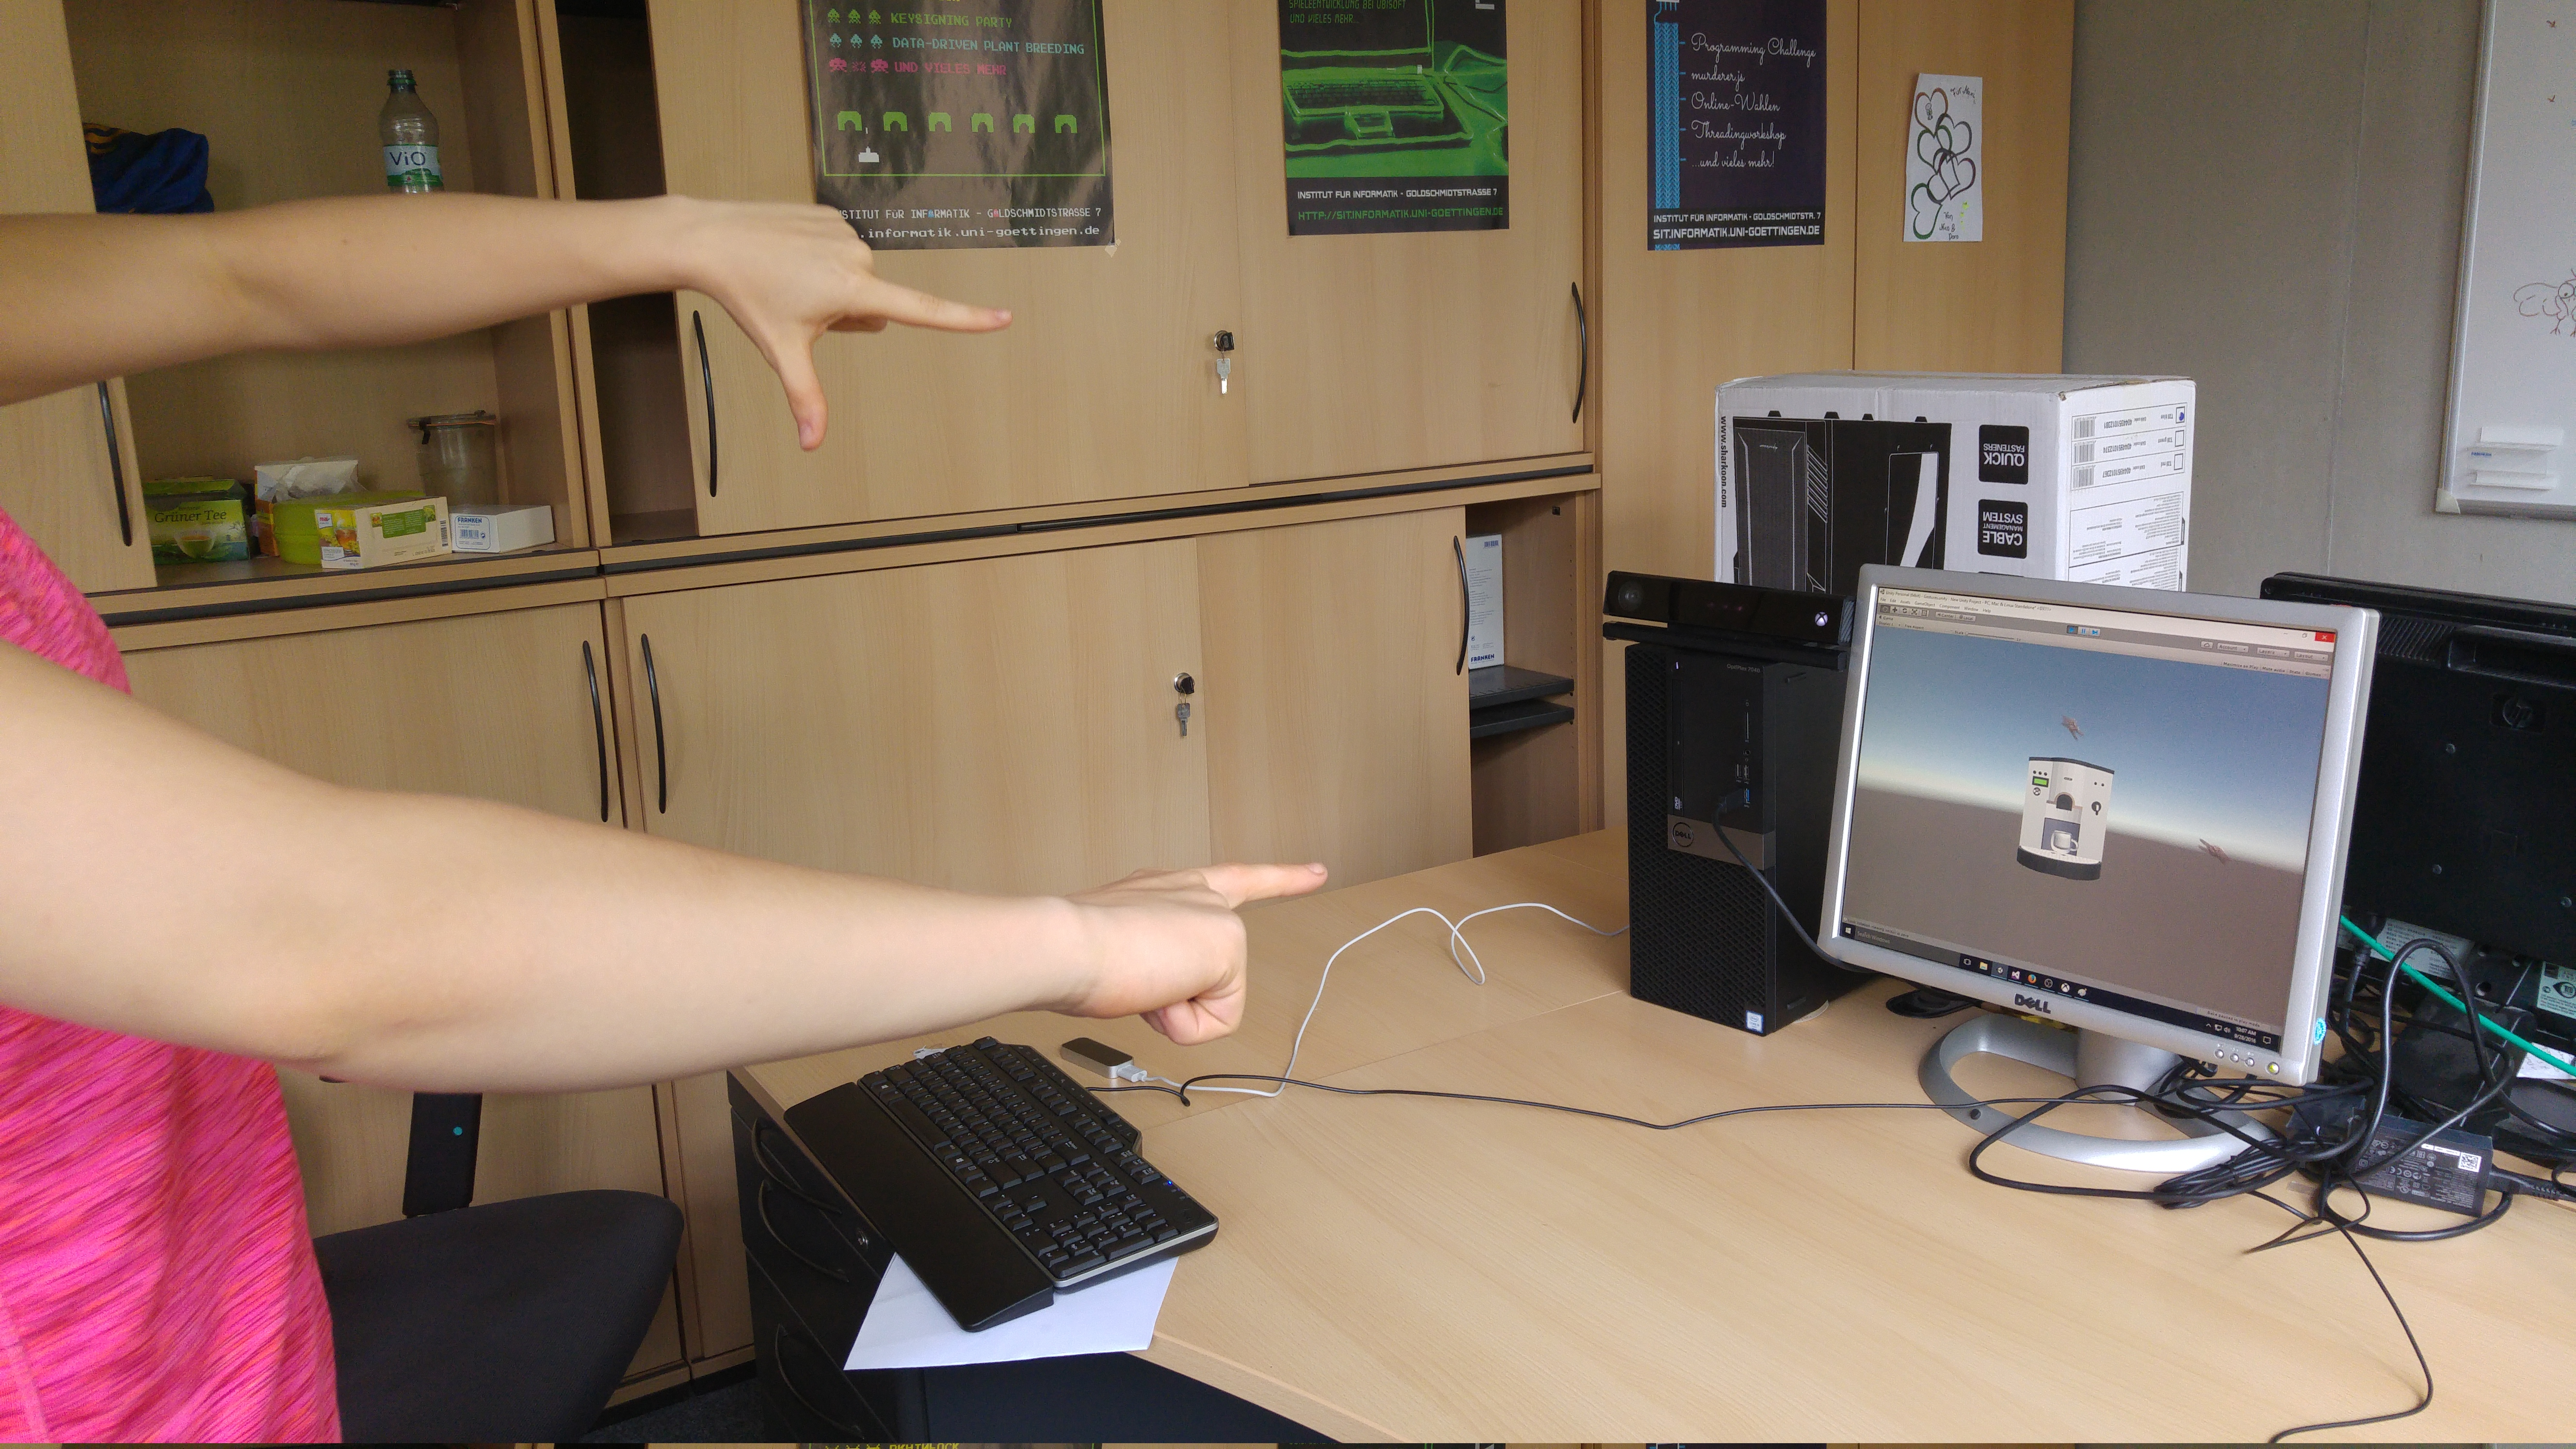
\includegraphics[width=\textwidth]{./figures/using_scene.jpg}
\caption{A user interacting with the scene.}
\end{figure}



- screenshot kinect usage of CM\\
- screenshot leap usage of CM\\
- precision of the used technologies\\


\chapter{Discussion}
Apart from the problems mentioned above we were astonished how quickly we were able to use our setup, move hand models via the Kinect in Unity3D and implement collision detection. Even though some things were a bit tricky, the software works quite well and can - for easy purposes - be almost used as plug-and-play.
Unfortunately this can't be said for the software available for Linux PCs, Windows is in the lead here. 


Of course there are several possibilities to further improve our project, some of them already mentioned above as well, e.g. the different frame selection or the fused usage of the Leap and Kinect.
Our setting also might have been not ideal, e.g. the placement of the Kinect next to and not on top of the screen and the relatively small distances between the Kinect sensors and the hands. 

It would also be a nice thing to stream the image of the screen to a smartphone and use a Google Cardboard to create the full virtual reality effect.
A  Google Cardboard is a cheap device where you can put your smartphone in and - by holding it in front of your eyes and with the help of the build-in sensors of the phone - experience virtual reality.
This could improve the usage of objects like our coffee machine even more and make it feel and look a bit more real.\\
\\
The whole virtual reality business is becoming increasingly important and is used more and more in our everyday life, so there are lots of projects and researches going on concerning this topic.
Just to mention a few: there is the so called social virtual reality with its virtual reality chatrooms, of course there are computer games using VR, but it could also be used for medical treatments, e.g. exposure therapies \cite{medicine}.


\chapter{Conclusion}
- possible to fuse data usefully\\
- possible to create a usable interaction this an object\\


%\appendix

\chapter{Additional}
\nocite{*} % Print all references regardless of whether they were cited in the poster or not
\bibliographystyle{plain} % Plain referencing style
\bibliography{sample} % Use the example bibliography file sample.b

\end{document}

